\documentclass[9pt,twocolumn,twoside,lineno]{pnas-new}
% Use the lineno option to display guide line numbers if required.
% Note that the use of elements such as single-column equations
% may affect the guide line number alignment. 

%Many authors find it useful to organize their manuscripts with the following order of sections;  Title, Author Affiliation, Keywords, Abstract, Significance Statement, Results, Discussion, Materials and methods, Acknowledgments, and References. Other orders and headings are permitted.

\usepackage[super]{nth} %adds superscripts for things like 20th

\templatetype{pnasresearcharticle} % Choose template 
% {pnasresearcharticle} = Template for a two-column research article
% {pnasmathematics} = Template for a one-column mathematics article
% {pnasinvited} = Template for a PNAS invited submission

\title{The Changing Character of Banded and Local Rainfall in China, 1951-2007}

% Use letters for affiliations, numbers to show equal authorship (if applicable) and to indicate the corresponding author
\author[a,1]{Jesse Day}
\author[a]{Inez Fung} 
\author[b]{Weihan Liu}

\affil[a]{Department of Earth and Planetary Science, University of California Berkeley, 94103}
\affil[b]{College of Letters and Sciences, University of California Berkeley, 94103}

%\subsection*{Author Affiliations}

%Include department, institution, and complete address, with the ZIP/postal code, for each author. Use lower case letters to match authors with institutions, as shown in the example. Authors with an ORCID ID may supply this information at submission.

% Please give the surname of the lead author for the running footer
\leadauthor{Day} 

% Please add here a significance statement to explain the relevance of your work
\significancestatement{Past researchers report a \nth{20}-century change in rainfall in densely-populated eastern China commonly referred to as the ``South Flood-North Drought.''  We examine decadal changes in banded rainfall, a substantial and distinctive component of the East Asia's rainfall climatology that we expect to respond to large-scale forcing. A novel rainband tracking algorithm partitions maps of daily rainfall into banded and local components, and allows compilation of statistical frequency, latitude and intensity of rainbands. Our results may abet ``fingerprinting'' of the impact of different types of anthropogenic forcing (in particular, greenhouse gases versus aerosols) on East Asian rainfall.}

% Please include corresponding author, author contribution and author declaration information
\authorcontributions{J.D. developed the algorithm and produced data; J.D. and I.F. contributed equally to the interpretation of results; W.L. contributed to algorithm development; }
\authordeclaration{The authors declare no conflict of interest.}
\correspondingauthor{\textsuperscript{2}To whom correspondence should be addressed. E-mail: jessed@berkeley.edu}

% Keywords are not mandatory, but authors are strongly encouraged to provide them. If provided, please include two to five keywords, separated by the pipe symbol, e.g:
\keywords{East Asian Monsoon|Monsoons|Rainfall|Rainbands|New Methods} 

\begin{abstract}
The topography and continental configuration of East Asia favor the year-round existence of zonal storm tracks that extend thousands of miles from eastern China into the northwestern Pacific Ocean. In spring and summer, these rainbands intensify (the ``Meiyu Front'') and shift northward during an annual series of rainfall stages collectively known as the East Asian monsoon. We develop a novel method called the Rainband Detection Algorithm (RDA), which detects rainbands in maps of daily rainfall and quantifies their attributes, and classifies rainfall into banded and local components. By applying RDA to the APHRODITE data set over eastern China, we produce a daily catalog of all rainband occurrences during 1951-2007 (20,819 days total). The climatological progression of the East Asian summer monsoon is revealed in unprecedented fashion. Furthermore, our data set reveals the changing character of Chinese rainfall over the second half of the twentieth century and beginning of the twenty-first. Across eastern China, decadal changes are dominated by changes in banded rainfall. Decadal changes between 1951-1979 and 1980-2007, known in the Chinese literature as the ``South Flood-North Drought,'' were produced predominantly by changes in rainband frequency. In contrast, eastern China rainfall increased in intensity during the period 1994-2007 without an increase in frequency. These may reflect different types of external forcing.
\end{abstract}

\dates{This manuscript was compiled on \today}
\doi{\url{www.pnas.org/cgi/doi/10.1073/pnas.XXXXXXXXXX}}

\begin{document}

% Optional adjustment to line up main text (after abstract) of first page with line numbers, when using both lineno and twocolumn options.
% You should only change this length when you've finalised the article contents.
\verticaladjustment{-2pt}

\maketitle
\thispagestyle{firststyle}
\ifthenelse{\boolean{shortarticle}}{\ifthenelse{\boolean{singlecolumn}}{\abscontentformatted}{\abscontent}}{}

\dropcap{E}astern China receives about 60\% of its precipitation from May to August via the East Asian summer monsoon. The period of peak rainfall lasting from early June to mid-July is called ``Meiyu season'' (lit. ``plum rains,'' referring to the spectacular growth of plum blossoms in central China with the onset of heavy rains). During this time, heavy rainfall occurs in zonal bands resulting from frontal synoptic conditions (the ``Meiyu Front''). The rainfall climatology of Japan and Korea also features similar time periods, known as Baiu and Changma respectively. The contribution from these rainbands leads to a rainfall seasonality in the East Asian monsoon that is unique relative to other monsoon circulations \citep{Ding2005}. More generally, rainbands are a year-round feature of Asian rainfall, attributed to the interplay between the East Asian tropospheric jet and Tibetan Plateau \citep{Molnar2010,Sampe2010,Chen2014}.
		
	We present a recursive image processing algorithm, the Rainband Detection Algorithm (RDA), which locates rainbands in a daily precipitation map and quantifies their attributes. By applying this algorithm to aggregated weather station data from APHRODITE, we create a 57-year (1951-2007) daily database of rainband occurrences in China. Several authors have compiled information on the variability of the Meiyu front on decadal and even centennial timescales \citep{Chen2004,Ge2008,Xu2009}, but to our knowledge no previous author has compiled a multi-decadal daily catalog of events. Likewise, the contribution of banded rainfall to seasonal and yearly totals has never been quantified across a large sample of days. We hope that our results can complement existing studies that discuss the characteristics of China rainfall obtained from the satellite record \citep{Luo2009,Luo2011,Luo2013}.
	
	 All rainfall on each day is further characterized as belonging to a rainband (``banded'' rainfall) or outside of any band (``local'' rainfall). We believe that this classification scheme ultimately corresponds to different causal mechanisms: Banded rainfall reflects large-scale convergence due to frontal conditions, whereas local rainfall likely results from mechanisms with shorter length scales such as convective self-buoyancy and orographic rainfall. We cannot rule out that multiple mechanisms are capable of forming rainbands. For instance, westward propagating cyclone tracks in late summer sometimes produce zonal bands. However, in reference \cite{Day2015}, it was shown that the typical radius of East Asian summer monsoon storms is only 200-300 km, while mean yearly rainband length is about 1200 km (Figure~\ref{fig:hov_climo}). Thus, our data show that storms propagate zonally across large distances at all times of year in East Asia. We attribute this notable feature to persistent frontal conditions that favor large-scale convergence.
	 
	 The temporal extent of our data set allows us to examine potential decadal changes. It has been broadly reported that China experienced a long-term shift in the distribution of rainfall known as the ``South Flood-North Drought'' (SFND), where the Yangtze River Valley witnessed an uptick in flooding and northern China an increased susceptibility to drought beginning in the 1980 \citep{Hu1997,Gong2002,Nigam2013}. A permanent change would have major humanitarian impacts on densely-populated eastern China, where a sizable fraction of the population depends on agriculture for subsistence. Under such circumstances, it is vital to understand whether this pattern will strengthen under global warming, or represents only a temporary deviation from the mean. The RDA algorithm presented before allows for partitioning of rainfall changes between banded and local components, and also a further decomposition of changes in banded rainfall \textit{events} between frequency and intensity changes. These changes are not captured by other existing metrics of China rainfall, as shown subsequently. We hope that the accurate characterization of these decadal rainfall changes can reveal underlying mechanisms in future work.
	 	 
	The following manuscript first describes the functionality of the Rainband Detection Algorithm, and then presents the seasonal progression of both banded and local rainfall and the intensity and frequency of rainband events. We then investigate decadal change in these properties, and suggest in conclusion potential relationships between these changes and other observed large-scale changes in recent decades.
	
\section*{Rainband Detection Algorithm (RDA)}

	As mentioned in the introduction, rainbands formed by westerly storms are observed year-round in East China (defined hereafter as the subregion 105-123$^{\circ}$E and 20-40$^{\circ}$N). Rainbands are defined as a continuous chain of longitudinal rainfall maxima in excess of 10 mm day$^{-1}$ spanning at least 5$^{\circ}$ of longitude. This study employs the APHRODITE APHRO\_MA v1101 product \citep{Yatagai2012}, which contains daily rainfall maps of the study region at $.25^{\circ} \times .25^{\circ}$ resolution for each day from 1 January 1951 to 31 December 2007 (20,819 days total). On each day, RDA first performs a weighted linear fit of the latitude of maximum rainfall at each longitude, using intensity as weighting and discarding outliers far from the centroid of precipitation, and then recursively repeats the fit using an increasingly narrow window around the previous best guess (Figure S4). The exact algorithm is described in greater detail in \citep{Day2016}. Once a fit is achieved, the following key metrics are calculated:
				
 \begin{itemize}
	 
	\item \textit{Quality Score (Q)}: The fraction of daily total East China rainfall that falls within $2.5^{\circ}$ degrees of the best estimate line (Figure S3).
	 
	 \item \textit{Latitude}: The latitude of the best fit line at 115$^{\circ}$E. 
	 
	 \item \textit{Intensity}: Mean rainfall of all ``rainband points'' (any point along the best fit line where daily rainfall exceeds 5 mm day$^{-1}$).
	 
	 \item \textit{Length}: Total number of rainband points (units of degrees longitude)
	 
	 \item \textit{Width}: Mean distance between half-maxima ($int_{max}$/2) on either side of each rainband point (units of degrees latitude).
	 
\end{itemize}
	
	 In some cases two rainbands exist simultaneously, in which case the more intense of the two is termed ``primary,'' and the weaker ``secondary.'' Secondary rainbands are detected by first removing all ``banded rainfall'' associated with the primary rainband (defined as all rainfall falling within 4$^{\circ}$ of a rainband axis, and any other adjacent points where rainfall exceeds 10 mm day$^{-1}$; Figure S1). If two rainbands coexist, \textit{conditional} quality scores $Q_1$ and $Q_2$ are calculated. $Q_1$ is defined as the fraction of daily East China rainfall that fell within $2.5^{\circ}$ degrees of the primary rainband \textit{after removing secondary rainband rainfall}, and vice-versa for $Q_2$ (Figure S3).
	
\subsection*{Quality Control}

	After running the algorithm for all 20,819 days from 1 January 1951 to 31 December 2007, we obtained 11,228 days with at least one rainband and 1,116 days with two rainbands. Subsequently, we apply a quality control (QC) algorithm to eliminate days with poor fit, based on the quality scores $Q$, $Q_1$ and $Q_2$ as well as the ``Taiwan fraction'' $TW$, defined as the percentage of daily total East China rainfall falling over the island of Taiwan (roughly 120-$122^{\circ}$E and 22-$26^{\circ}$N). Rainband fits are deemed successful if they satisfy the following two criteria:

\begin{enumerate}

	\item $TW < 20\%$. If $TW > 20\%$, the day's fit is thrown out (238 cases total, 2.1\% of total fits). Such days are dominated by tropical storms reaching Taiwan and do not exhibit a strong rainband (example shown in Figure~\ref{fig:algo_3}a).  
	
	\item The quality scores of the fit must meet either of the two following benchmarks:
	
	\begin{enumerate} 
	
	\item If $Q>.6$, the fit is deemed successful (7,522 days, 67.0\% of total fits; Figure~\ref{fig:algo_3}b). If $Q_2$ is also greater than .6, the day will be classified as a double rainband day (Type I double rainband; 232 cases). 3.1\% of days where $Q>.6$ also achieve $Q_2>.6$.
		
	\item If $Q<.6$, the fit is discarded unless two rainbands are detected and both $Q_1 > .6\mathrm{\ \textbf{and}\ }Q_2 > .6$ (where again $Q_1$ and $Q_2$ are \textit{conditional} quality scores as defined above). In such cases, the presence of multiple rainbands of similar intensity initially obscures the goodness of fit (Figure~\ref{fig:algo_3}d). Such days are also classified as double rainband days (Type II double rainband; 466 cases).
	
	\end{enumerate}
	
	If neither criterion 2a nor 2b is satisfied, the fit is thrown out (Figure~\ref{fig:algo_3}c).
	
\end{enumerate}	

	The use of conditional quality scores $Q_1$ and $Q_2$ adds 466 double rainband fits (6.2\% of all successful fits) that would otherwise have been missed due to $Q<.6$. 33.2\% of double rainband days are Type I ($Q>.6$) and 66.8\% Type II ($Q<.6$) as defined above. Double rainbands are more common during certain months, particularly July-September. Supplementary Tables S1-S3 contain detailed results of the application of RDA to years 1951-2007 in APHRODITE.

\subsection*{Rainfall Types}
	
	RDA allows us to classify all rainfall on each day as either \textit{banded} (falls within a rainband) or \textit{local}. \textit{Banded} rainfall consists of all rainfall falling within 4$^{\circ}$ of a rainband axis and any other adjacent points where rainfall exceeds 10 mm day$^{-1}$, the same definition as in step 5 of the recursive algorithm above. An example is shown in Figure~\ref{fig:algo_4}a. Rainfall on each of the 20,819 available days was partitioned into its banded and local components. This allows us to determine what fraction of rainfall at each point in East China is supplied via banded rainfall (Figure~\ref{fig:type_climo}). We also test for the significance of decadal changes in banded and local rainfall separately (Figure~\ref{fig:type_changes}). 

%%FIGURE 1 Hovm�ller diagram of Meiyu latitude occupancy, 1951-2007. Produced by MATLAB scripts meiyufig1.m and meiyustats_compact.m.
\begin{figure}[htbp]
\centering
\noindent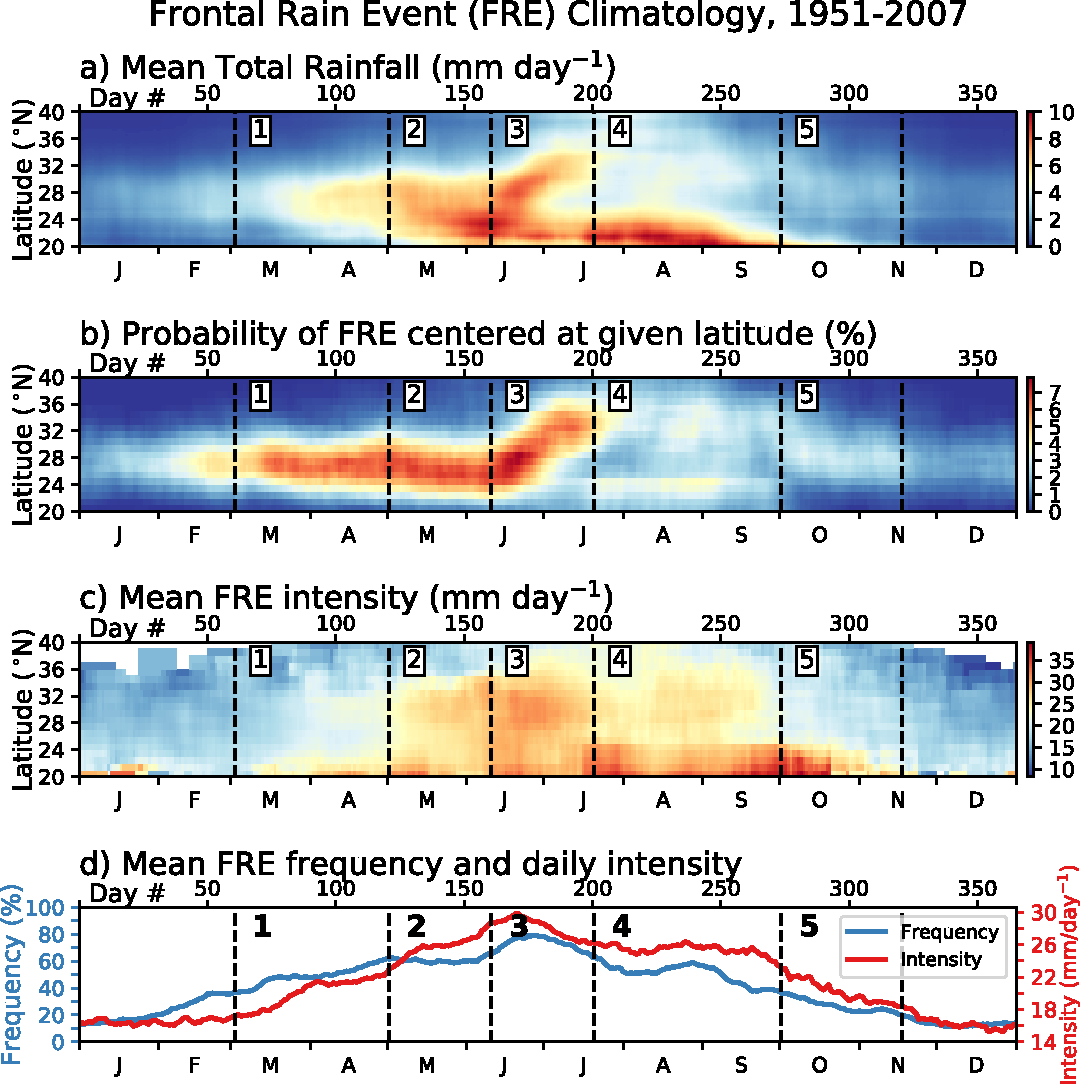
\includegraphics[width=\linewidth]{Figures/PNAS_climo}
\caption{Climatology of East Asian rainfall and rainbands, 1951-2007, with important time periods marked as follows: 1 - Spring Rains; 2 - Pre-Meiyu; 3 - Meiyu; 4 - Post-Meiyu; 5 - Fall Rains. a) Hovm\"oller diagram of precipitation (100-123$^{\circ}$E longitudinal average); b) Hovm\"oller diagram of absolute probability of observing a rainband (both primary and secondary), smoothed in time with a 9-day and 2$^{\circ}$-running box filter; c) Probability of primary rainband occurrence and mean intensity (9-day running mean); d) The conditional probability of a secondary rainband given the presence of a primary rainband, as well as the mean tilt and length of primary rainband events (9-day running mean).}
\label{fig:hov_climo}
\end{figure}

\section*{Results}

\subsection*{Rainband Climatology}

	We compile our daily rainband catalog into a 57-year daily climatology (1951-2007). Abrupt climatological shifts occur simultaneously in both rainfall and rainband climatology. We define 5 periods of distinct behavior as demarcated in Figure~\ref{fig:hov_climo}, with the Pre-Meiyu, Meiyu and Post-Meiyu equivalent to the three stages of Meiyu rainfall described in reference \cite{Ding2005}.

\begin{enumerate}

\item The Spring Rains (days 60-120, March 1-April 30), previously studied in reference \cite{Tian1998}, marked by frequent but relatively weak rainbands (47\% occurrence, 20 mm day$^{-1}$ mean);

\item Pre-Meiyu season (days 121-160, May 1-June 9), during which rainfall and front intensity steadily increase (56\% occurrence, 25.5 mm day$^{-1}$ mean);

\item Meiyu season (days 161-200, June 10-July 19) when a remarkable 7-degree northward shift in mean rainband latitude occurs over the course of several weeks, and rainband frequency and intensity peaks (66\% occurrence, 28.3 mm day$^{-1}$ mean); 

\item Post-Meiyu season (days 201-273, July 20-September 30), when rainbands are less common than during the Spring Rains (42\% occurrence) but double rainbands occur more frequently (28\% chance of observing a secondary rainband if a primary rainband is observed); 

\item The Fall Rains (days 274-320, October 1-November 16), when mean rainband latitude shifts back southward from its northern maximum of 30$^\circ$N and rainband frequency decreases to just 27\%. 

\end{enumerate}

%%FIGURE 2 Decadal mean in different rainfall types during different time periods
\begin{figure}[htb]
\centering
\noindent\includegraphics[width=\linewidth]{Figures/RDA_type_climo_topo}
\caption{Climatology of the amount of total rainfall, banded rainfall and local rainfall for the full year, Pre-Meiyu (days 121-160), Meiyu (days 161-200) and Post-Meiyu (days 201-273). \textit{Banded} rainfall consists of all rainfall falling within 4$^{\circ}$ of a rainband axis and rainfall at any other adjacent point exceeding 10 mm day$^{-1}$. \textit{Local} rainfall includes all rainfall not meeting these criteria. Note that color bar switches from .5 to 1 mm day$^{-1}$ increment past 5 mm day$^{-1}$.}
\label{fig:type_climo}
\end{figure}


	The total number of rainband counts as well as the mean and standard deviation of rainband frequency, latitude and intensity during each time period are presented in Table S4. These results are comparable with the frontal event catalog of \cite{Xu2009}, who analyzed Meiyu rainbands in TRMM data for 1998-2007 and found a similar date for the northward transition of the Meiyu front. 

	The yearly progression of precipitation over eastern China is shown in Figure~\ref{fig:hov_climo}a, longitudinally averaged over $100-123^\circ$E with a 5-day running mean, similar to \cite{Ding2005}. Unlike other monsoonal regions, which tend to be very dry in winter \citep{Wang2002}, Eastern China receives about 40\% of yearly precipitation between September and April. Though these time periods are chosen subjectively, we also reproduce our analysis in the form of Hovm\"oller plots of climatology and decadal differences, which confirm our analysis.
	
	Figure~\ref{fig:hov_climo}b shows a Hovm\"oller diagram of the probability of rainband occurrence at each latitude, including both primary and secondary rainbands. The transition from Pre-Meiyu to Meiyu and from Meiyu to Post-Meiyu both entail a rapid northward migration in rainfall (Figure~\ref{fig:hov_climo}b) and abrupt changes in rainband statistics (Figure~\ref{fig:hov_climo}b). The onset of the Meiyu is marked by a climatological jump both in rainband frequency and intensity around day 160 (June 9) that persists for 20 days when rainbands are concentrated between 26$^\circ$ and 30$^\circ$N. Yet by day 200 (July 19), this same region is less likely than any other latitude to feature a rainband, featuring roughly an 80\% local decline in rainband frequency and a decline in total rainfall from 7.6 mm day$^{-1}$ (days 161-180 mean) to 4.1 mm day$^{-1}$ (days 201-220 mean).
	
	Figure~\ref{fig:hov_climo}c shows the probability of rainband occurrence and mean intensity on each day. Frontal rainbands over China can appear in any month, with their probability of occurrence and intensity maximizing in late June (80\% probability of occurrence, mean intensity of 31 mm day$^{-1}$) and minimizing in January (10\% probability occurrence, mean intensity of 12 mm day$^{-1}$). Rainbands are generally more probable and stronger during spring than in fall, with notable intensity jumps around days 120 and 160. Some periods of heavy rainfall, in particular the August peak over southern China (over 10 mm day$^{-1}$ around 20$^{\circ}$N), do not correspond to a surge in rainband frequency. Instead, August and September are known as the months when northwestern Pacific typhoons reach mainland China, which tends to leave locally favorable rainfall conditions in their wake \citep{Chen2007,Chen2011}. The most intense rainbands registered occur at low latitudes during October (days 270-300), likely corresponding to peak cyclone season \citep{Liu2003}. Figure~\ref{fig:hov_climo}d shows mean rainband tilt and length, as well as the conditional probability of observing a secondary rainband given the presence of a primary rainband. 
	
\subsubsection*{Banded vs Local Rainfall}	
	
	Figure~\ref{fig:type_climo} shows that banded rainfall constitutes at least 40\% of yearly total for all of mainland China east of 105$^\circ$E between 21$^\circ$N and 37$^\circ$N, over 60\% for most of central China, and up to 74\% in the vicinity of Jiangxi Province (28$^\circ$N, 116$^\circ$E). Thus, banded rainfall is an essential component of East China's yearly rainfall budget. Banded rainfall constitutes the majority of rainfall during the Pre-Meiyu and Meiyu, but not the Post-Meiyu. 

	Banded rainfall undergoes a dramatic progression previously evidenced in Figure~\ref{fig:hov_climo}. In contrast, local rainfall retains a similar spatial configuration from season to season, with regions of local rainfall anchored by topography. For instance, a recurrent rainy band is visible along the southern edge of the South China/Qinling mountains. The Sichuan Basin also shows up as a locus of local rainfall; previous studies have shown that Sichuan experiences an unusual local rainfall climatology due to being directly in the lee of the Tibetan Plateau. Banded rainfall only constitutes a noticeable fraction of Taiwanese rainfall during the Pre-Meiyu. In fact, the term Meiyu season as used in Taiwan is typically centered around late May, although our study defines the Meiyu as June 10-July 19 \citep{Chen1994,Xu2009}.

%%FIGURE 3 Decadal changes in different rainfall types
\verb|
\begin{figure*}[!htp]
\centering
\noindent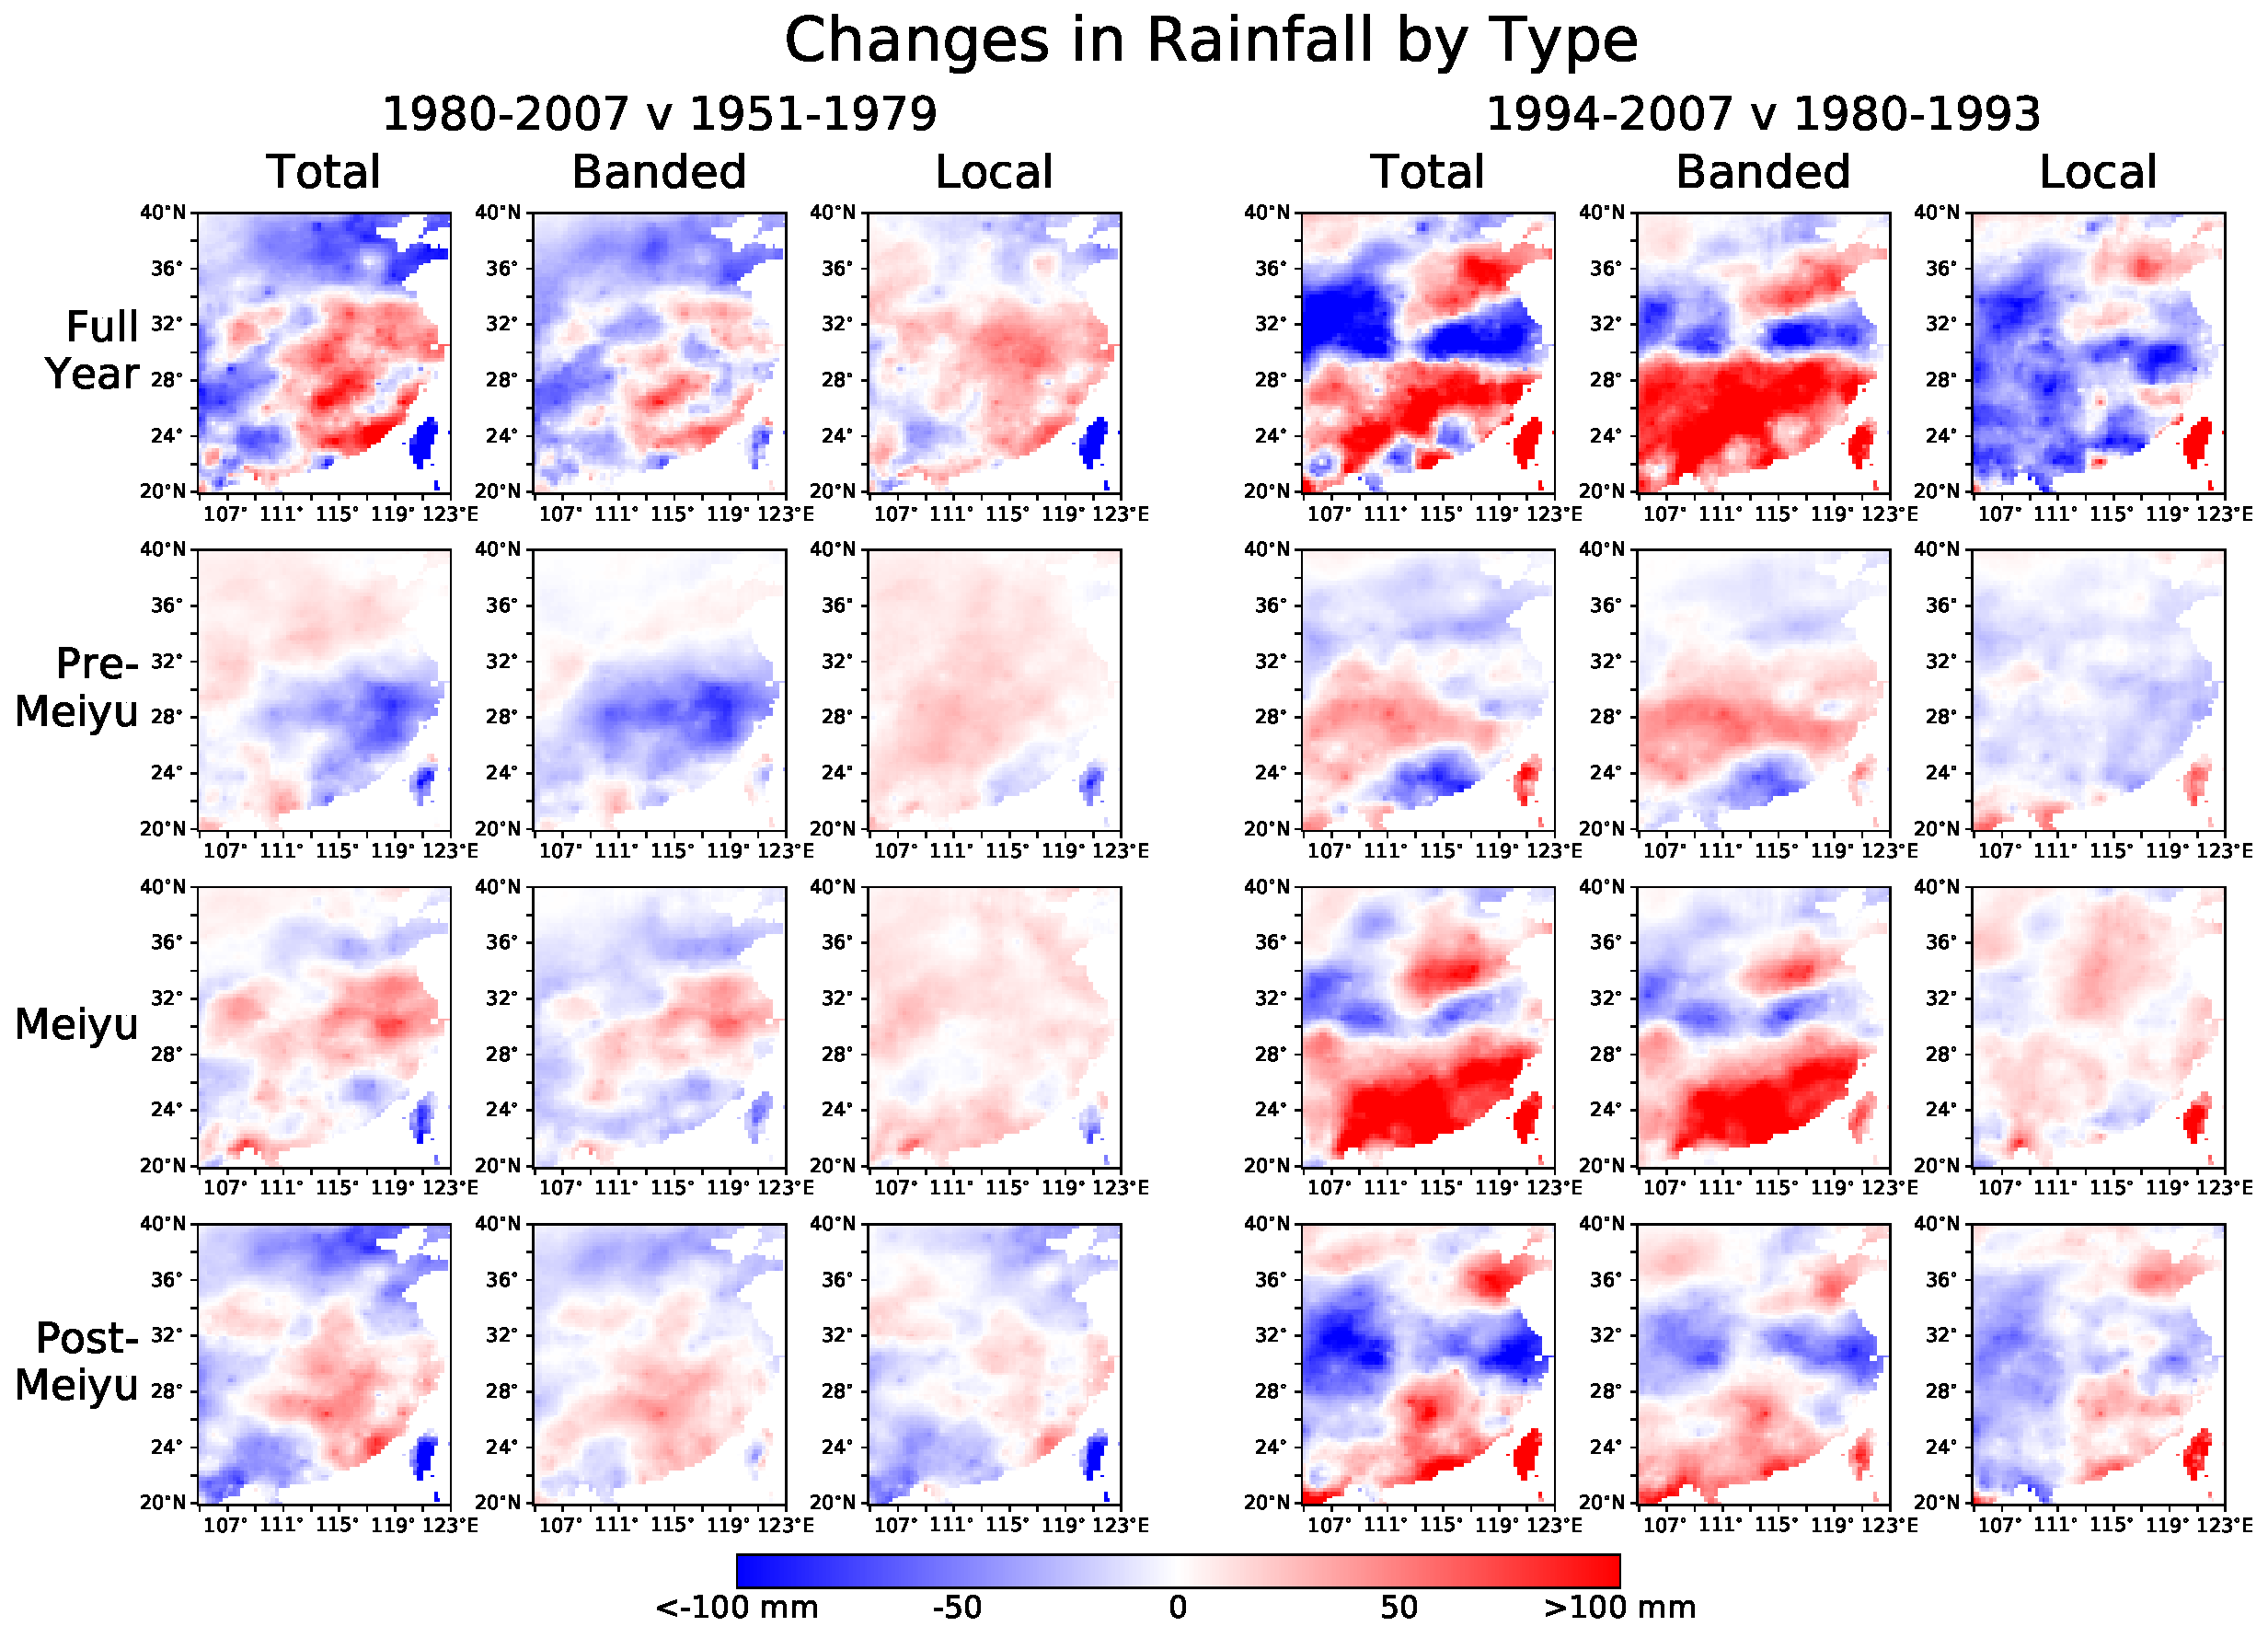
\includegraphics[width=11.4cm]{Figures/changes_by_type}
\caption{Changes in total, banded and local rainfall for full year, Pre-Meiyu (days 121-160), Meiyu (days 161-200) and Post-Meiyu (days 201-273), comparing time periods 1980-2007 to 1951-1979 (left) and 1994-2007 to 1980-1993 (right).
Significance changes at the 95\%/99\% level are marked by single/double hatches (permutation test with 1,000 iterations). \textit{Banded} rainfall consists of all rainfall falling within 4$^{\circ}$ of a rainband axis and rainfall at any other adjacent point exceeding 10 mm day$^{-1}$. \textit{Local} rainfall includes all rainfall not meeting these criteria.}
\label{fig:type_changes}
\end{figure*}|

\section*{Decadal Changes}

\subsection*{1980-2007 versus 1951-1979}

	China experienced a well-known ``South Flood-North Drought'' pattern of rainfall change between the mid- and late-\nth{20} century. The yearly mean change in rainfall rate between 1951-1979 and 1980-2007 over the region 100$^{\circ}$-142$^{\circ}$E and 20$^{\circ}$-48$^{\circ}$N is shown in Figure~\ref{fig:type_changes}. The South Flood-North Drought refers in particular to a meridional dipole of decadal rainfall change over eastern China (110$^{\circ}$-125$^{\circ}$E and 22$^{\circ}$-42$^{\circ}$N), where most of China's population resides. Pronounced local shifts are also visible in Taiwan, South Korea and parts of Japan. This work focuses on eastern China. Annual changes in northern China between 35$^{\circ}$-40$^{\circ}$N are significant at a 95\% confidence level, whereas changes in central and southern China are not. However, there are substantial changes in central and southern China rainfall during particular Meiyu stages, as discussed below.
	
	Using RDA to partition daily rainfall into its banded and local components, we can quantify how much changes in each type of rainfall have contributed to total change. Figure~\ref{fig:type_changes} compares banded and local rainfall changes between the periods 1980-2007 and 1951-1979 over the whole year, and also during the Pre-Meiyu, Meiyu and Post-Meiyu seasons. Northern China has seen a major decrease in total rainfall (significant at a 99\% level), due in largest part to a decline in banded rainfall during the Post-Meiyu. Also, during the Pre-Meiyu season, a marked decrease in banded rainfall over the Yangtze River Valley ($p<.005$) is partially offset by a general increase in local rainfall across all of China, especially in the vicinity of Hunan, Guizhou and Chongqing Provinces (108$^\circ$-114$^\circ$E, 26$^\circ$-30$^\circ$N). Generally, banded and local rainfall changes are uncorrelated. Figure~\ref{fig:hov_changes} shows some significant changes also in winter rainfall, but the biggest rainy season changes are clearly due to changes in banded rainfall.

	Having isolated banded rainfall as the cause of decadal rainfall changes between 1980-2007 and 1951-1979, we can further attribute the change to a change in rainband frequency, intensity, or both. Figure~\ref{fig:hov_changes}) shows a H\"ovmoller plot of changes in frequency and intensity for the entire year, with only changes significant at a 95\% level shown. The most coherent significant changes in rainband frequency occur during the pre-Meiyu around 30$^\circ$N, and during the post-Meiyu around 35$^\circ$N, while there are no concerted changes in intensity during the warm rainy period (some are visible during the cold season). 
	
	Analyzing more closely by time period, we find that during the Pre-Meiyu (days 121-160), the average probability of observing a primary rainband has declined from $59.0\% \pm 2.0\%$ to $53.0\% \pm 2.1\%$ ($p=0.020$; Figure~\ref{fig:bars} which we estimate as producing an XXX mm/day decline in rainfall. This Pre-Meiyu decrease in rainfall was previously identified by several authors \citep{Xin2006,Wang2009}. For the Post-Meiyu (days 201-273, or July 20-Sep 30), we specifically analyze rainbands occurring north of 27$^{\circ}$N, since rainbands in southern China during this time period are likely produced by typhoons, distinct from other mechanisms of rainband formation. Mean rainband latitude during 1951-1979 was $33.6^\circ \textrm{N} \pm .3^\circ$ for events north of 27$^{\circ}$N, versus $32.9^\circ \textrm{N} \pm .3^\circ$ during 1980-2007 ($p=.0003$; Figure~\ref{fig:bars}). This shift remains significant if we do not restrict by front latitude ($p=.0048$). As a result, yearly rainfall has increased in central China even though Pre-Meiyu rainfall changes in that region are actually negative (Figure~\ref{fig:hov_changes}). Unlike reference \cite{Yu2010}, our catalog does not exhibit a \nth{20}-century decreasing trend in the intensity of Yangtze River region frontal rainbands during July-August. A significant southward shift in rainband latitude is also found for the whole year ($p=.0032$; Figure~\ref{fig:bars}), but this signal is dominated by the Post-Meiyu shift.
	
%%FIGURE 4 Significance of attribute changes in rainbands between decades
\begin{figure}[htbp]
\centering
\noindent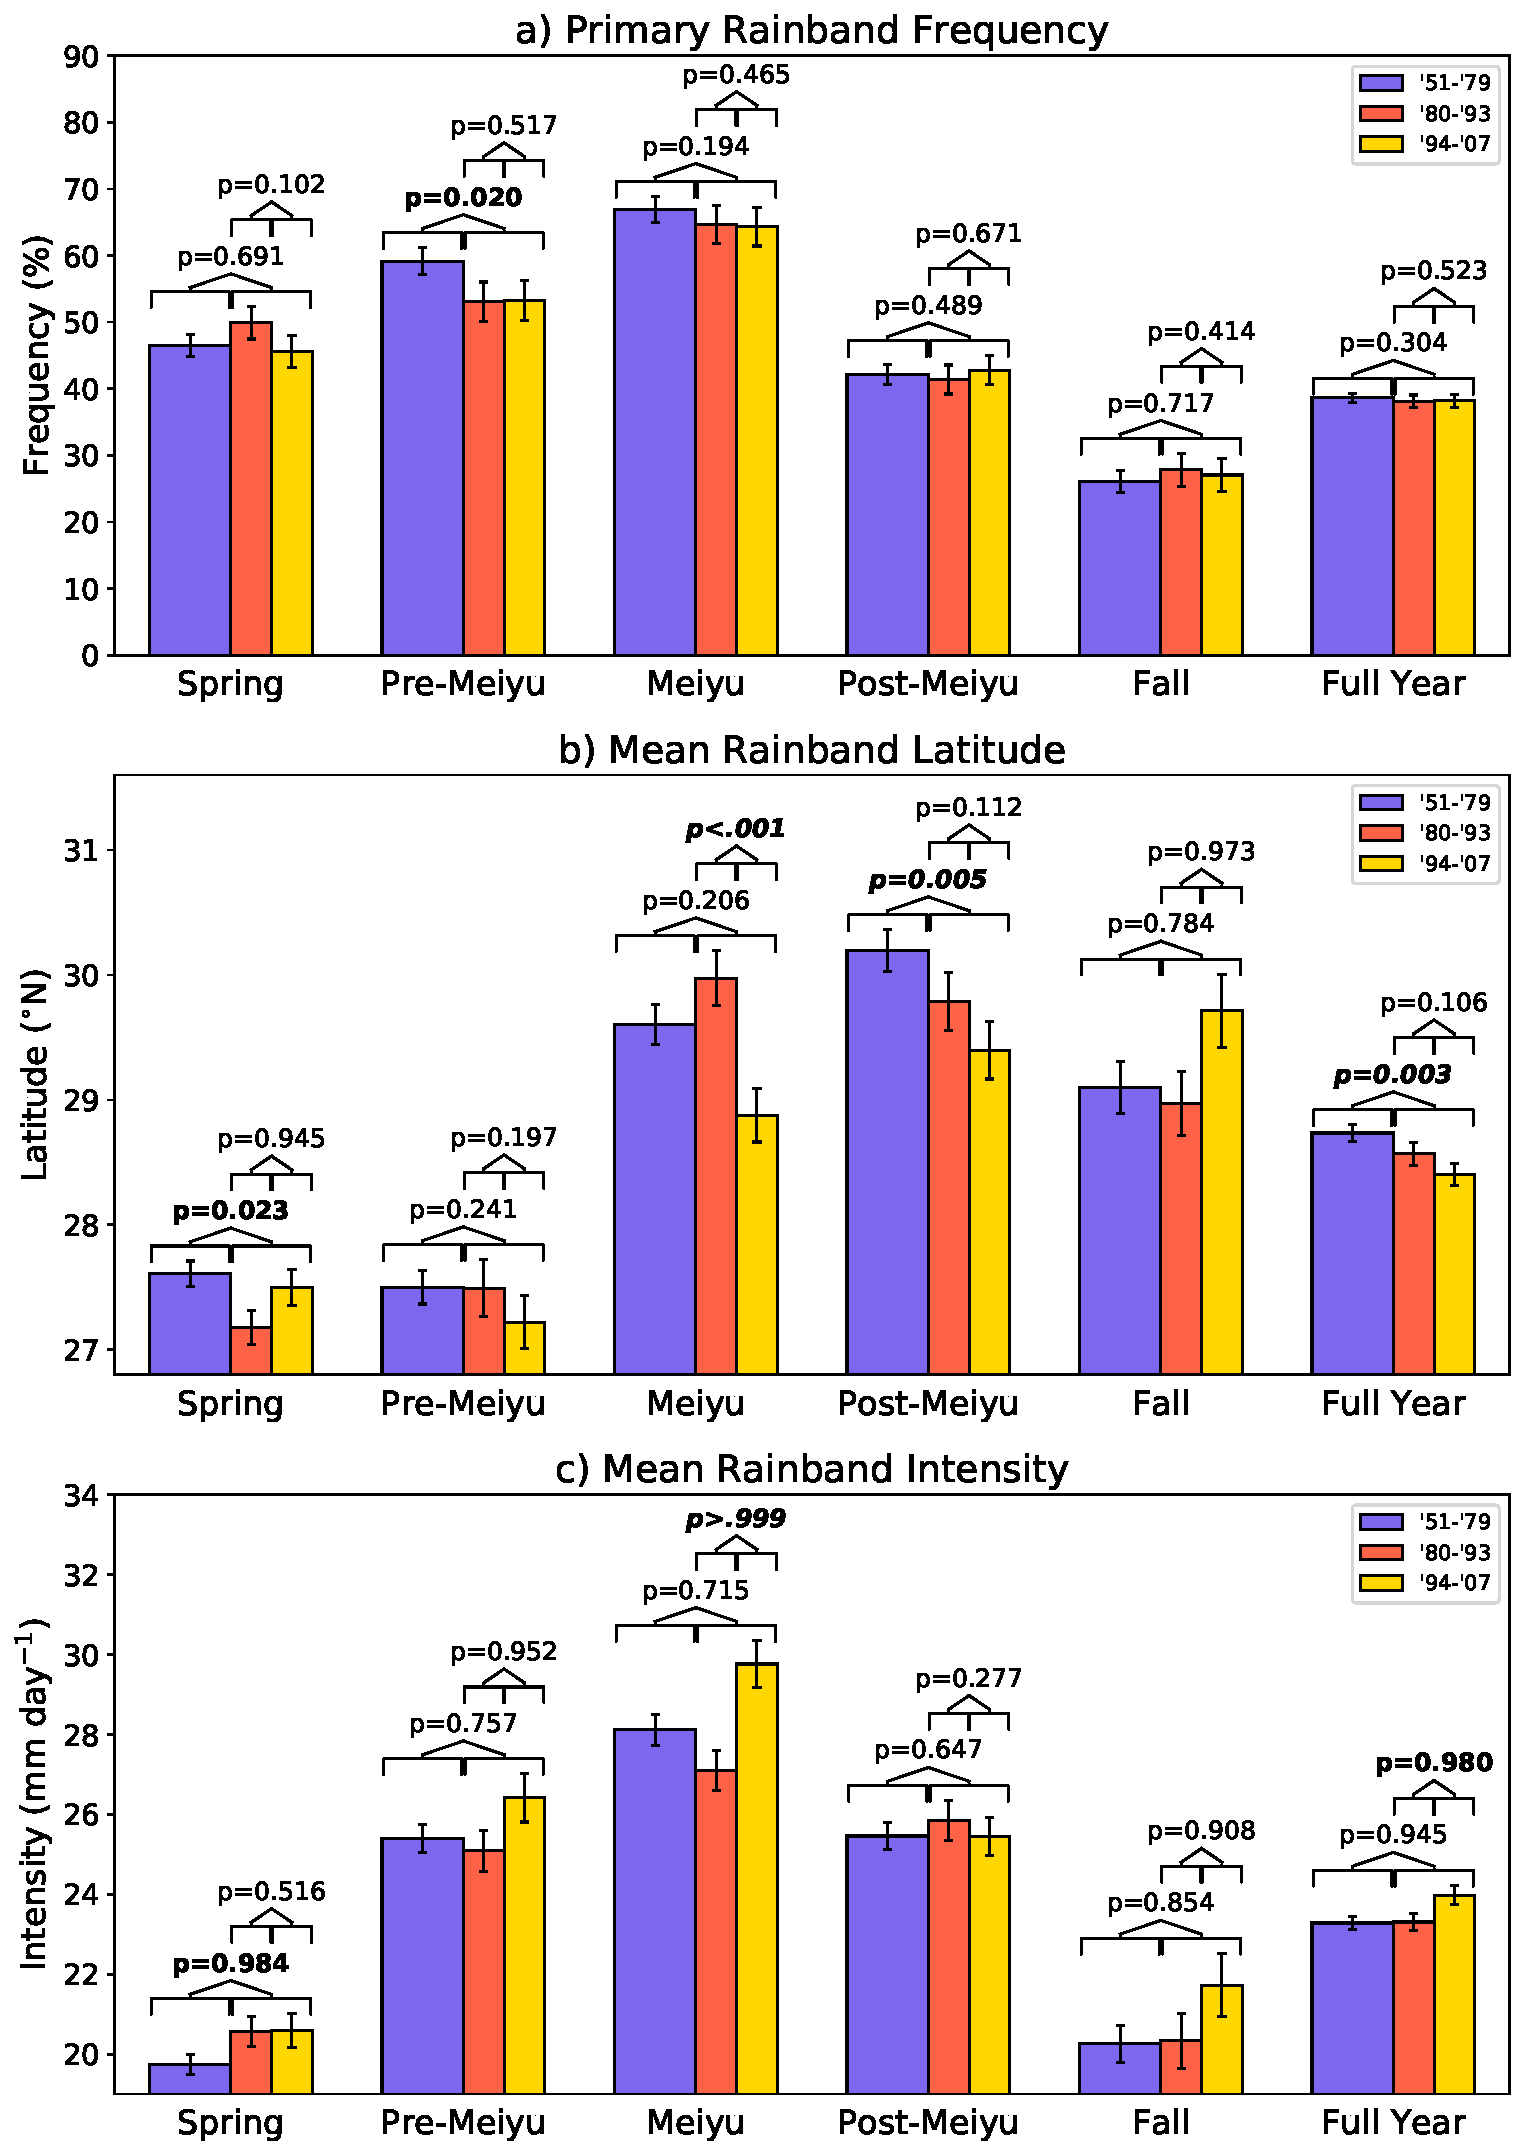
\includegraphics[width=\linewidth]{Figures/bars}
\caption{Significance of decadal changes in a) Rainband frequency, b) Rainband latitude and c) Rainband intensity between decades.}
\label{fig:bars}
\end{figure}	

	We verify these results by testing the significance of the changes in \textit{distribution} during 1980-2007 relative to 1951-1979 using bootstrap Kolmogorov-Smirnov (KS) and Anderson-Dearing (AD) tests. Neither test captures the Pre-Meiyu decline in rainband frequency after 1979 since rainband latitude and intensity distributions remain similar. On the other hand, the Post-Meiyu southward shift in rainband latitude is found to be highly significant by both tests ($p<.001$). As before, no significant changes in rainband intensity are found between 1951-1979 and 1980-2007. This suggests that the estimates of significance from permutation testing are trustworthy.
	
	We have also compared metrics $M_1-M_8$ between 1980-2007 and 1951-1979 for the whole year and during each of the five Meiyu stages described above. Very few significant changes are found. The most notable change is a significant decrease in $M_5$ (North China Rainfall) for both the full year and Post-Meiyu, in concurrence with our findings in Figure~\ref{fig:type_changes}. The highly significant decrease in central China rainfall during the Pre-Meiyu and increase during the Post-Meiyu are not captured by any of the alternative metrics, and the metrics also cannot reflect the observed zonal symmetry. We conclude that the use of RDA captures key features of the South Flood-North Drought that are not revealed by analyzing simpler metrics.
	
	In summary, the RDA method partitions Chinese rainfall into useful components, banded and local, each with distinct spatial and temporal distributions. Decadal changes in banded and local rainfall feature distinct spatial patterns. The South Flood-North Drought pattern of change between 1980-2007 and 1951-1979 can be attributed primarily to changes in banded rainfall, and more specifically to changes in the frequency of rainband occurrence.
	
\subsection*{1980-1993 versus 1994-2007}
	
	We repeat the methodology described above with the set of years 1994-2007 versus 1980-1993, when past authors have reported a shift in South China rainfall \citep{Kwon2007,Wu2010,Yim2013}. Changes between these two time periods are shown in Figure~\ref{fig:type_changes}. The spatial pattern of change during 1980-1993 versus 1994-2007 is distinct from that shown in 1980-2007 versus 1951-1979. Specifically, the former resembles a zonally symmetric tripole, whereas the latter resembles more of a dipole pattern. These are known to be the leading modes of eastern China rainfall variability \citep{Day2015}.
	
	Figure~\ref{fig:hov_changes} shows that, unlike the 1980-2007 versus 1951-1979 comparison, significant summer changes occur in both banded and local rainfall, especially in July and August. Rainbands have generally intensified year round, and especially during the pre-Meiyu and Meiyu seasons over southern China. In particular, during Meiyu season, mean rainband latitude shifted southward from $30.0^\circ \textrm{N} \pm .4^\circ$ to $28.9^\circ \textrm{N} \pm .4^\circ\ (p=.0002)$ and the \textit{intensity} of rainbands also jumped from $27.3 \pm 1.1$ mm day$^{-1}$ to $29.8 \pm 1.1$ mm day$^{-1}\ (p=.9994)$, leading to increased rainfall over central and southern China. \cite{Zou2015} also found that China experienced a more intense Meiyu during the 1990s, as well as generally more severe rainfall events. Unlike the comparison between 1951-1979 and 1980-2007, rainband \textit{frequency} remained unchanged. Testing for the significance of the change in distribution, both the KS and AD tests found an altered distribution of intensity and latitude of rainbands during Meiyu season during 1994-2007 relative to 1980-1993, with $p<.001$ for both changes\citep{Day2016}.
	
	In summary, the changes in rainfall between 1980-1993 and 1994-2007 are fundamentally different from the South Flood-North Drought pattern of changes between 1951-1979 and 1980-2007. In the former case, both banded and local rainfall experienced significant changes, and the change in banded rainfall was marked by a change in \textit{intensity}. During the latter, changes in the frequency of rainbands (without a change in intensity) led to decreases in banded rainfall. We propose that these two distinct kinds of decadal change reflect different forcing mechanisms, as explored in the conclusion.
	
	Other regions with distinct rainfall subclimates such as the Sichuan Basin and Taiwan have also undergone significant decadal changes in local rainfall independent from the rest of eastern China in which changes in local rainfall play an important role, further suggesting the utility of rainfall classification based on RDA.
	
%%FIGURE 5 Changes in rainfall by type in Hovmoller form
\verb|
\begin{figure*}[htbp]
\centering
\noindent
\includegraphics[width=17.6cm]{Figures/hov_summary}
\caption{15-day running mean of the change in a) total rainfall; b) banded rainfall; c) rainband frequency and d) rainband intensity, zonally averaged by latitude over 110-123$^{\circ}$E, comparing years 1980-2007 to 1951-1979 (left) and 1994-2007 to 1980-1993 (right). All changes shown are significant at a 95\% level, and significance exceeding a 99\% level is contoured in gray, as calculated by a moving blocks bootstrap with block length of 2 days and 2,000 iterations. Zonal rainfall averages \textit{exclude} rainfall occurring over Taiwan because the magnitude of changes over the island dwarf changes on the mainland.}
\label{fig:hov_changes}
\end{figure*}|

\section*{Conclusion}

	This work has aimed to quantify the role of frontal storms in the yearly rainfall climatology of eastern China. We used the Rainband Detection Algorithm (RDA), a recursive image processing algorithm, to compile a 57-year catalog of daily rainband occurrence over China and the properties of each event, such as latitude, intensity, tilt, width and length. Over 50\% of yearly total precipitation is contributed by banded rainfall in most of eastern China. We identify a sequence of 5 stages of frontal precipitation, each with preferred position, frequency and strength of frontal rainfall: 1) the Spring Rains (March 1-April 30); 2) the Pre-Meiyu (May 1-June 9); 3) the Meiyu (June 10-July 19); 4) the Post-Meiyu (July 20-September 30) and 5) the Fall Rains (October 1-November 16) (Figure~\ref{fig:hov_climo}). The climatological transitions from one period to the next are marked by sharp changes in rainband frequency, latitude and intensity. Simpler alternative metrics of eastern China rainfall fail to reproduce most of these features. Banded rainfall peaks during Meiyu season (late June), while local rainfall peaks during the Post-Meiyu (early August). We argue that these reflect different causal mechanisms (large-scale convergence versus local heating).
	
	Decadal changes in rainfall in eastern China are primarily due to changes in banded rainfall, as opposed to local rainfall (Figures~\ref{fig:type_changes}). A decrease in northern China rainband \textit{frequency} was the principal contributor to drought during 1980-2007 relative to 1951-1979 (Figure~\ref{fig:hov_changes}; $p=<.001$). The start of the rainy season over the Yangtze Valley was also postponed due to a decline in rainband frequency ($p=0.02$). Changes during 1994-2007 versus a 1980-1993 baseline are instead dominated by rainband \textit{intensity} changes during Meiyu season with no change in frequency ($p>.999$). We suggest that the two shifts detailed in this study may result from two different causal mechanisms.
	
	Past authors have attributed these decadal rainfall changes to a combination of anthropogenic forcing\citep{Xu2001,Li2010,Zhao2010,Song2014} and natural variability\citep{Zhang1999,Xin2006,Ding2008,Zhou2009,Qu2012,Lei2014}. In particular, authors have focused on the proliferation of black carbon aerosols in conjunction with Asia's industrialization \citep{Menon2002,Fan2012,Streets2013}. High PM10 aerosol concentration (diameter l $<\mu m$) has been correlated with increased medium-to-heavy rainfall and decreased light rainfall \citep{Choi2008,Wang2016}, possibly linked to the intensity changes shown in this study. Global warming may also affect the East Asian monsoon via other climate components including Pacific and Indian Ocean SST \citep{Gong2002}, the ENSO cycle \citep{Xie2010} and the annual cycle East Asian tropical jet \citep{Yu2007, Archer2008,Park2014,Park2014a,Chiang2015}.
	
	It is essential to understand whether the South Flood-North Drought pattern will persist under \nth{21}-century warming \citep{Zhang1999,Xin2006,Lei2014}. The CMIP5 (Climate Model Intercomparison Project) model suite contained in the Intergovernmental Panel on Climate Change's Fifth Assessment Report (IPCC AR5) does not agree on the sign of future summer rainfall changes in East Asia \citep{Christensen2011}. Depending on the relative roles of global warming, aerosols and natural variability in the East China rainfall changes studied in this paper, anomalies may be exacerbated or return to their \nth{20} century baseline. Since anthropogenic aerosol concentration is projected to decline during the \nth{21} century \citep{Westervelt2015}, the effects of continued global warming will predominate, potentially with a distinct "thumbprint" of rainfall intensity and frequency changes \citep{Trenberth2011a,Pendergrass2014b,Wang2016}. Improved attribution of \nth{20}-century East China rainfall changes may therefore improve future projections.

%\begin{table}%[tbhp]
%\centering
%\caption{Comparison of the fitted potential energy surfaces and ab initio benchmark electronic energy calculations}
%\begin{tabular}{lrrr}
%Species & CBS & CV & G3 \\
%\midrule
%1. Acetaldehyde & 0.0 & 0.0 & 0.0 \\
%2. Vinyl alcohol & 9.1 & 9.6 & 13.5 \\
%3. Hydroxyethylidene & 50.8 & 51.2 & 54.0\\
%\bottomrule
%\end{tabular}

%\addtabletext{nomenclature for the TSs refers to the numbered species in the table.}
%\end{table}

\matmethods{
\subsection*{APHRODITE Rainfall}

	The APHRO\_MA\_V1101 product from APHRODITE (Asian Precipitation - Highly-Resolved Observational Data Integration Towards Evaluation of the Water Resources) includes 57 years (1951-2007) of continental daily rainfall (PRECIP product) on a .25$^{\circ} \times .25^{\circ}$ grid over 60$^{\circ}$-150$^{\circ}$E and 15$^{\circ}$S-55$^{\circ}$N \citep{Yatagai2012}, as well as a daily map of reporting weather stations on the same grid (RSTN product). Values are reported over land only. We focus on the subregion inside of 105$^{\circ}$E-123$^{\circ}$E and 20$^{\circ}$N-40$^{\circ}$N where rainbands are known to occur frequently, especially during Meiyu season (early June to late July). The network of stations remains dense (100-200 km spacing) through time, such that rainbands are clearly resolved and we are not concerned about potential artifacts from changes in station density. APHRODITE's resolution cannot capture some features visible in TRMM satellite data \citep{Xu2009}, but its length allows for the study of decadal change. We use the words ``rainfall'' and ``precipitation'' interchangeably in the rest of this work since most precipitation consists of rain, although snow is common in northeastern China during winter.
}

\showmatmethods % Display the Materials and Methods section

\acknow{	APHRODITE precipitation data is publicly available at \url{http://www.chikyu.ac.jp/precip/index.html}. The rainband detection algorithm was written in MATLAB and subsequent data analysis carried out within Jupyter Notebook. The author's data analysis is freely available on Github. Ferret, a NOAA product, was used for some figure generation and is freely available at \url{http://ferret.pmel.noaa.gov/Ferret/}. A full database of rainband statistics from 1 January 1951 to 31 December 2007 and associated MATLAB and Ferret codes used to produce results are available on the author's Github repository. This work was supported by NSF grants EAR-0909195 and EAR-1211925, which allowed the presentation of preliminary results in conference settings, as well as DOE grant DE-SC0014078. We also acknowledge NSFC (National Natural Science Foundation of China) grant \#40921120406 for enabling our collaboration with Professor Yanjun Cai of IEECAS in Xi'an, which led to the present work. We thank Jinqiang Chen and an anonymous reviewer for valuable suggestions on a previous version of this manuscript.}

\showacknow % Display the acknowledgments section

% \pnasbreak splits and balances the columns before the references.
% If you see unexpected formatting errors, try commenting out this line
% as it can run into problems with floats and footnotes on the final page.
\pnasbreak

% Bibliography
\bibliography{RDA_biblio}

\end{document}